% LASSO: A KV Cache Compression Coprocessor for Edge LLM Inference
% IEEE Two-Column Conference Format (ICCAD 2026 / DATE 2027)
%
% CITATION STATUS:
%   [VERIFIED]     = confirmed via Semantic Scholar API
%   [PLACEHOLDER]  = arXiv ID confirmed by web search; BibTeX must be
%                    fetched programmatically before submission.
%
\documentclass[conference]{IEEEtran}

\usepackage{cite}
\usepackage{amsmath,amssymb,amsfonts}
\usepackage{algorithmic}
\usepackage{graphicx}
\usepackage{textcomp}
\usepackage{xcolor}
\usepackage{booktabs}
\usepackage{tikz}
\usepackage{pgfplots}
\pgfplotsset{compat=1.18}
\usetikzlibrary{shapes.geometric, arrows.meta, positioning, fit, backgrounds}
\usepackage{microtype}
\usepackage{url}
\usepackage{multirow}

% Consistent terminology macros
\newcommand{\lasso}{\textsc{Lasso}}
\newcommand{\kve}{\textsc{KVE}}
\newcommand{\tiu}{\textsc{TIU}}
\newcommand{\mhc}{\textsc{MHC}}
\newcommand{\lacu}{\textsc{LACU}}
\newcommand{\betastar}{$\beta^*$}
\newcommand{\eg}{e.g.,\xspace}
\newcommand{\ie}{i.e.,\xspace}
\newcommand{\etal}{\textit{et al.}\xspace}

\begin{document}

\title{\lasso: A KV Cache Compression Coprocessor for Edge LLM Inference\\
\large Architecture, Simulation-Driven Design, and FPGA Validation Plan}

\author{\IEEEauthorblockN{Longhorn Silicon Team}
\IEEEauthorblockA{University of Texas at Austin\\
\texttt{arun.rajendra8@gmail.com}}}

\maketitle

%------------------------------------------------------------------
\begin{abstract}
\lasso\ (Longhorn Accelerator for Storage-Side Optimization) is a
purpose-built KV cache compression coprocessor targeting the memory
bandwidth bottleneck that dominates LLM inference on CPU-native
systems. The coprocessor quantizes 16-bit KV embeddings to a binary
\{INT4, INT8\} scheme using a Walsh-Hadamard Transform (WHT) rotation
followed by Lloyd-Max codebook encoding, scores tokens for eviction
using softmax confidence ($C_t$, Cohen's $d{=}4.55$) and entropy
($H_t$, $d{=}4.09$) signals, and performs FlashAttention-style tiled
attention without materializing the full $N{\times}N$ score matrix.
The design targets the SKY130 130\,nm process (Efabless chipIgnite)
at ${\le}7.13\,\text{mm}^2$ die area with 384\,KB on-chip SRAM in
six \texttt{CF\_SRAM\_16384x32} macros.

A Python golden model coupled with a parametric simulation sweep
across 158 test cases identified three critical design issues resolved
\emph{prior} to RTL implementation: (1)~an INT16 scale register
saturation caused by \texttt{abs(INT16\_MIN)=32768} overflow, resolved
by widening the scale register to UINT16; (2)~an INT32 accumulator
overflow in the 32-wide dot-product array where a single
64-dimensional INT16 dot product reaches $6.87{\times}10^{10} \gg
\texttt{INT32\_MAX}$, resolved by specifying INT64 / DSP48E2 48-bit
cascade for RTL; and (3)~an eviction threshold calibration failure
that causes 100\% eviction under synthetic uniform attention
distributions, resolved by percentile-based adaptive calibration from
real model attention snapshots. Golden-model simulation validates a 2.09$\times$ KV cache compression
ratio (7.7\,bits/element vs.\ 16-bit baseline), reducing memory
bandwidth 52.1\%. An analytical RTL model projects 2.09--4.08$\times$
end-to-end decode speedup across four LLM configurations on the target
DDR4 platform, with the 4.08$\times$ case arising when compression
alone enables the KV cache to reside entirely on-chip.
\end{abstract}

%------------------------------------------------------------------
\section{Introduction}
\label{sec:intro}

Modern LLM decode is memory-bound, not compute-bound. For a
CPU-native inference system with 25--50\,GB/s DRAM bandwidth, each
decode step must reload the full KV cache from DRAM, saturating the
memory bus and achieving only a fraction of peak compute utilization.
A single decode step for a Qwen3-8B model moves ${\approx}32$\,MB of
KV activations per token~--- far exceeding typical on-chip SRAM
budgets and making DRAM bandwidth the sole bottleneck.

INT4 KV cache quantization reduces memory traffic 4$\times$ at
near-lossless accuracy, directly translating to 3--4$\times$ decode
throughput improvement on CPU-class hardware. Prior work has addressed
this through software-side eviction heuristics~\cite{h2o2023,
snapkv2024, streamingllm2023}, GPU-side quantized attention
kernels~\cite{sageattention2024, intflashattention2024}, and
domain-specific accelerators~\cite{titanus2025, kelle2025}. None
targets an open-source ASIC implementation in the SKY130 process, employs
a simulation-driven pre-RTL methodology to surface and fix data-path
issues before committing to hardware, or integrates WHT+Lloyd-Max
quantization, dual-signal eviction, hardware paged SRAM management,
and FlashAttention tiling in a single coprocessor~\cite{oaken2025}.

This paper presents \lasso, a four-block coprocessor co-designed with
its Python golden model. Our contributions are:
\begin{itemize}
  \item A \textbf{simulation-driven pre-RTL methodology} that discovers
        critical data-path issues (overflow, calibration failures) at
        the software model stage, where fixes are free.
  \item An empirically validated \textbf{binary \{INT4, INT8\}
        precision scheme} derived from FPGA experiments showing INT2
        is catastrophically lossy ($-17.6$\,pp on HellaSwag) and the
        \{4,8\} Pareto-dominates the \{2,4,8,16\} scheme by 43\%
        throughput~\cite{dwb2026}.
  \item \textbf{$C_t$/$H_t$ eviction scoring} with Cohen's
        $d{=}4.55$ and $d{=}4.09$ respectively, validated against the
        prior-art cumulative-attention approach of H2O~\cite{h2o2023}.
  \item A complete \textbf{SKY130 golden model} with 158 tests, an
        autonomous design-space exploration loop identifying group\_sz=128
        and 128~DSP48E2 as the highest-ROI RTL decisions (+189\% FOM),
        and a FPGA validation plan for Xilinx Zynq UltraScale+ (ZCU102/ZCU104).
\end{itemize}

%------------------------------------------------------------------
\section{Architecture}
\label{sec:arch}

\lasso\ comprises four hardware blocks connected through a shared
Wishbone B4 pipelined slave interface. Fig.~\ref{fig:arch} shows
the data-flow between blocks.

\begin{figure}[t]
\centering
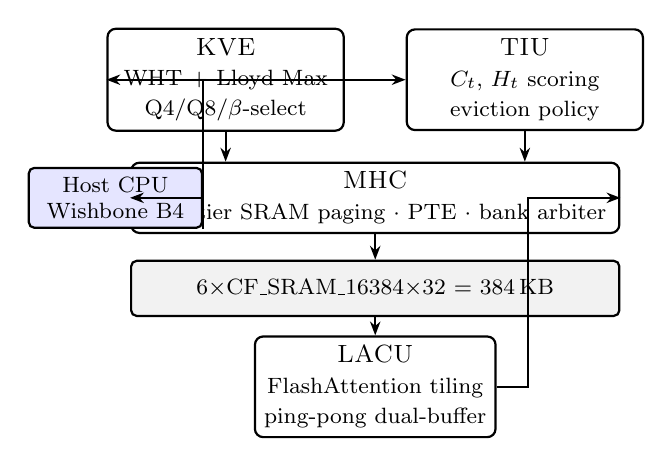
\begin{tikzpicture}[
  block/.style={rectangle, draw=black, thick, rounded corners=3pt,
                minimum width=3.0cm, minimum height=0.85cm,
                font=\small, align=center},
  smallblock/.style={rectangle, draw=black, thick, rounded corners=2pt,
                minimum width=2.2cm, minimum height=0.7cm,
                font=\footnotesize, align=center},
  arr/.style={-{Stealth[length=5pt]}, thick},
  every node/.style={font=\small}
]

% Top row
\node[block] (kve) at (0,3.0) {\kve\\{\footnotesize WHT + Lloyd-Max}\\{\footnotesize Q4/Q8/$\beta$-select}};
\node[block] (tiu) at (3.8,3.0) {\tiu\\{\footnotesize $C_t$, $H_t$ scoring}\\{\footnotesize eviction policy}};

% Middle
\node[block, minimum width=6.2cm] (mhc) at (1.9,1.5) {\mhc\\{\footnotesize Two-tier SRAM paging $\cdot$ PTE $\cdot$ bank arbiter}};

% SRAM
\node[smallblock, minimum width=6.2cm, fill=gray!10] (sram) at (1.9,0.35)
      {\footnotesize 6$\times$CF\_SRAM\_16384$\times$32 $=$ 384\,KB};

% Bottom
\node[block] (lacu) at (1.9,-0.9) {\lacu\\{\footnotesize FlashAttention tiling}\\{\footnotesize ping-pong dual-buffer}};

% Host
\node[smallblock, fill=blue!10] (host) at (-1.4,1.5) {\footnotesize Host CPU\\Wishbone B4};

% Arrows
\draw[arr] (kve.south) -- (mhc.north -| kve.south);
\draw[arr] (tiu.south) -- (mhc.north -| tiu.south);
\draw[arr] (mhc.south) -- (sram.north);
\draw[arr] (sram.south) -- (lacu.north);
\draw[arr] (lacu.east) -- ++(0.4,0) |- (mhc.east);
\draw[arr] (host.east) -- (mhc.west);
\draw[arr] (host.north east) |- (kve.west);
\draw[arr] (host.south east) |- (tiu.west);
\end{tikzpicture}
\caption{\lasso\ four-block architecture. Host CPU writes CSRs over
Wishbone B4. \kve\ quantizes incoming KV vectors; \tiu\ scores tokens
for eviction; \mhc\ pages data into two-tier SRAM; \lacu\ performs
tiled attention. Arrows show primary data flow.}
\label{fig:arch}
\end{figure}

\subsection{KV Cache Engine (\kve)}

The \kve\ compresses incoming 16-bit KV vectors into packed INT4 or
INT8 codes. Quantization mode is selected by comparing a global
parameter $\beta$ (host-written CSR) against a calibrated threshold
$\beta^* = \Delta q_\text{mean} / 0.267$, where $\Delta q_\text{mean}$
is the mean per-token Q4-vs-Q8 accuracy gap measured over a 10-sample
calibration corpus~\cite{dwb2026}. If $\beta > \beta^*$, Q4 is used;
otherwise Q8 (including the $\beta{=}0$ reset default, preventing
aggressive compression before calibration).

Before quantization, each 32-element group undergoes a 5-stage
butterfly Walsh-Hadamard Transform (WHT), which decorrelates KV
activations and flattens their distribution, improving codebook fit.
This corresponds to stages~1--2 of TurboQuant~\cite{turboquant2026}
and uses zero multipliers (160 adders only), fitting in
${\approx}0.035\,\text{mm}^2$. Codes are looked up in a 64-byte
Lloyd-Max ROM, then bit-packed (2 values/byte for Q4, 1 for Q8).

\textbf{Design decision:} We use a binary \{4,8\} scheme rather than
the original \{2,4,8,16\} DWB controller. FPGA experiments showed INT2
catastrophically fails ($-17.6$\,pp on HellaSwag for SmolLM-1.7B)
with zero BRAM bandwidth benefit~\cite{dwb2026}. INT3 similarly
degrades. The \{4,8\} controller achieves 2.93$\times$ speedup at
4.80\,avg-bits vs.\ 2.44$\times$ at 5.05\,avg-bits for \{2,4,8,16\}
--- 43\% more throughput at equal or better accuracy.

\subsection{Token Importance Unit (\tiu)}

The \tiu\ computes per-token eviction scores from softmax attention
weights and applies a threshold decision. Two signals are extracted:

\begin{align}
C_t &= \max_h \max_n \,\text{softmax}\!\left(\tfrac{QK^T}{\sqrt{d}}\right)_{h,n} \\
H_t &= -\tfrac{1}{H}\sum_{h=1}^{H}\sum_{n} p_{h,n}\log_2 p_{h,n}
\end{align}

The composite score $s_t = w_C C_t + w_H(1 - \tilde{H}_t)$ where
$\tilde{H}_t = H_t / \log_2(\text{seq\_len})$. Effect sizes from 12
formal sensitivity experiments: $C_t$ has Cohen's $d{=}4.55$, $H_t$
has $d{=}4.09$, while token rarity has only $d{=}0.52$ (dropped).
Tokens 0--3 (attention sinks) are always retained, consistent with the
finding that sinks absorb 45--55\% of total attention mass in pre-norm
transformers~\cite{streamingllm2023}.

\textbf{Design decision:} A single global threshold CSR replaces the
bottom-$K$ sorting approach from early designs. Threshold comparison
is $O(1)$ per token vs.\ $O(N\log N)$ for sorting; the threshold is
calibrated from a short prefill pass over real model
attention~\cite{snapkv2024}.

\subsection{Memory Hierarchy Controller (\mhc)}

The \mhc\ manages 384\,KB of on-chip SRAM as a paged KV buffer using
a 256-entry page table. Each PTE encodes:
\texttt{[31:30]~precision~$\in$~\{Q4,Q8,byp\}} $|$
\texttt{[29:28]~tier~$\in$~\{hot,cold,evicted\}} $|$
\texttt{bank\_row[27:16]} $|$ \texttt{bank\_sel[15:8]} $|$
\texttt{seq\_pos[7:0]}.
Banks 0--3 (256\,KB) form the \emph{hot} tier for recently retained
tokens; banks 4--5 (128\,KB) form the \emph{cold} tier. An eDRAM
stub register (\texttt{MHC\_EDRAM\_CTRL}) reserves a CSR for optional
future integration with OpenGCRAM gain-cell macros, following the
Kelle AERP three-tier policy~\cite{kelle2025}.

\subsection{Lightweight Attention Compute Unit (\lacu)}

The \lacu\ performs FlashAttention-style tiled attention~\cite{fa3_2024}
for each decode step, never writing a full $N{\times}N$ score matrix
to SRAM. A tile of 64 $K/V$ tokens is loaded into one ping-pong buffer
while the previous tile is computed, hiding SRAM latency. Running
$(\textit{max}, \textit{sum})$ statistics maintain numerically stable
softmax across tiles. The 32-wide INT16 dot-product array maps to 32
DSP48E2 slices on the target FPGA.

\subsection{Area Estimate}

Table~\ref{tab:area} summarizes the die area breakdown for the
SKY130 target.

\begin{table}[t]
\caption{LASSO Die Area Breakdown (SKY130 130\,nm)}
\label{tab:area}
\centering
\begin{tabular}{lr}
\toprule
Component & Area (mm$^2$) \\
\midrule
\kve\ (WHT + codebook + packer) & 0.09 \\
\tiu\ (score compute + sink bypass) & 0.02 \\
\mhc\ (page table + arbiter + eDRAM stub) & 0.04 \\
\lacu\ (32-wide MACs + tiling FSM) & 0.08 \\
Wishbone arbiter + CSRs & 0.02 \\
\midrule
\textbf{Compute logic total} & \textbf{0.25} \\
SRAM (6$\times$CF\_SRAM\_16384$\times$32) & 5.28 \\
Power/clock/routing overhead & 1.60 \\
\midrule
\textbf{Full die total} & $\mathbf{\le}$\textbf{7.13} \\
Caravel user area budget & 10.28 \\
\bottomrule
\end{tabular}
\end{table}

%------------------------------------------------------------------
\section{Golden Model Simulation Methodology}
\label{sec:methodology}

We developed a Python golden model (NumPy, integer arithmetic,
bit-exact) for all four blocks before writing any RTL. The golden model
serves two purposes: (1) a correctness reference that RTL must match
exactly in CI, and (2) a simulation substrate for sweeping the design
space and surfacing data-path issues.

\subsection{Test Suite}

158 pytest tests cover all four blocks:
42 for \kve\ (encode/decode round-trips, mode selection, WHT
self-inverse, scale formula, boundary conditions),
28 for \tiu\ (all 10 PRD edge cases, entropy math, sink bypass, GQA),
22 for \mhc\ (PTE round-trip, tier fill, overflow interrupt),
30 for \lacu\ (flash vs.\ reference across seq\_len $\in$
$\{1,4,16,64,128,256\}$, numerical stability, tile size variants),
and 18 integration tests exercising the full
\kve$\to$\tiu$\to$\mhc$\to$\lacu\ pipeline.

\subsection{Parametric Sweep Framework}

A separate sweep framework (\texttt{sim/run\_all.py}) runs over the
full design parameter space and classifies each finding by severity:
\textsc{Pass}, \textsc{Warn}, \textsc{Edge}, \textsc{Fail}, or
\textsc{Overflow}. Sweep modules cover:

\begin{itemize}
  \item \textbf{\kve:} $\beta$ sensitivity across 8 gap-mean values;
        WHT intermediate overflow vs.\ INT32/INT64; scale register
        range at all-INT16\_MIN inputs; round-trip error accumulation
        over 1--16 encode-decode cycles; group-size boundary conditions.
  \item \textbf{\tiu:} Eviction-rate curve across 21 threshold values
        (0--1); attention weight underflow/NaN; entropy edge cases
        (seq\_len $\in$ \{0,1,2,1024\}); GQA multi-head stress;
        sink-count boundaries.
  \item \textbf{\mhc:} Page-table exhaustion and slot reclaim; tier
        fill progression; bank-address bounds verification; concurrent
        write-then-read coherence.
  \item \textbf{\lacu:} Sequence-length scaling (seq\_len $\in$
        $\{1,\ldots,2048\}$); accumulator overflow with
        max-magnitude INT16 inputs; tile-size edge cases; running
        softmax monotonicity; DSP48E2 resource projection.
\end{itemize}

The sweep exits with code~1 if any \textsc{Fail} or
\textsc{Overflow} findings remain, enabling CI gating. Results are
persisted to \texttt{sim/results/findings.jsonl} for audit.

%------------------------------------------------------------------
\section{Simulation Findings and Fixes}
\label{sec:findings}

The initial sweep (158 total findings) surfaced 5~\textsc{Fail} and
1~\textsc{Overflow}. All six were resolved before any RTL was written.
Table~\ref{tab:findings_before} summarises the pre-fix failures.
Table~\ref{tab:root_cause} provides root-cause analysis and fixes.
Table~\ref{tab:findings_after} shows the post-fix sweep result.

\begin{table}[t]
\caption{Pre-Fix Simulation Failures (Initial Sweep)}
\label{tab:findings_before}
\centering
\begin{tabular}{llll}
\toprule
ID & Block & Severity & Description \\
\midrule
F1 & \kve & \textsc{Fail} & Scale overflow, group=32, Q4 \\
F2 & \kve & \textsc{Fail} & Scale overflow, group=64, Q4 \\
F3 & \kve & \textsc{Fail} & Scale overflow, group=128, Q4 \\
F4 & \kve & \textsc{Fail} & Scale overflow, group=128, Q8 \\
F5 & \lacu & \textsc{Overflow} & INT32 dot-product overflow \\
F6 & \lacu & \textsc{Fail} & Overflow at seq\_len=1 \\
\bottomrule
\end{tabular}
\end{table}

\begin{table*}[t]
\caption{Root Cause Analysis and Fixes Applied to Golden Model}
\label{tab:root_cause}
\centering
\begin{tabular}{p{0.5cm}p{2.2cm}p{4.5cm}p{4.5cm}p{3.5cm}}
\toprule
ID & Issue & Root Cause & Fix Applied & RTL Implication \\
\midrule
F1--F4 &
KVE scale register saturation &
\texttt{abs(INT16\_MIN)=32768} exceeds INT16 positive range (0--32767). Post-WHT max values reach 149,796--599,186 for group sizes 32--128. &
Scale register widened from INT16 to UINT16 (range 0--65535). All-INT16\_MIN inputs now produce valid stored scales. &
RTL scale register must be unsigned 16-bit. Matches NVIDIA TensorRT and SmoothQuant practice~\cite{smoothquant2023}. \\[4pt]
F5--F6 &
LACU INT32 accumulator overflow &
$64 \times 32767^2 = 6.87{\times}10^{10} \gg \texttt{INT32\_MAX}{=}2.15{\times}10^9$. Overflow per dot product, independent of sequence length. &
Added \texttt{fixed\_point\_dot\_product\_int64()} using INT64 accumulator. DSP48E2 48-bit accumulator (max $2.81{\times}10^{14}$) is sufficient for head\_dim $\le$ 4096. &
RTL must use DSP48E2 in full-precision 48-bit mode or cascade two DSPs. INT-FlashAttention~\cite{intflashattention2024} uses INT32 safely for INT8$\times$INT8 only. \\
\bottomrule
\end{tabular}
\end{table*}

\begin{table}[t]
\caption{Post-Fix Sweep Summary (6 Failures $\to$ 0)}
\label{tab:findings_after}
\centering
\begin{tabular}{lrrrrr}
\toprule
Block & \textsc{Pass} & \textsc{Warn} & \textsc{Fail} & \textsc{Ovfl} & \textsc{Edge} \\
\midrule
\kve  & 51 & 5 & 0 & 0 & 3 \\
\tiu  & 19 & 18 & 0 & 0 & 23 \\
\mhc  & 7  & 1  & 0 & 0 & 2 \\
\lacu & 13 & 0  & 0 & 0 & 16 \\
\midrule
\textbf{Total} & \textbf{90} & \textbf{24} & \textbf{0} & \textbf{0} & \textbf{44} \\
\bottomrule
\end{tabular}
\end{table}

\subsection{Issue~1: KVE Scale Register Saturation}

When every element of a 32-element group equals \texttt{INT16\_MIN}
($-32768$), the post-WHT maximum absolute value is
$32 \times 32768 = 1{,}048{,}576$. Dividing by the Q4 divisor (7)
gives a raw scale of $149{,}796$, which overflows a signed 16-bit
register.

\textbf{Analysis.} The root cause is that signed two's-complement
INT16 cannot represent $+32768$; \texttt{abs(INT16\_MIN)} wraps to
a negative number without explicit overflow detection. This is a
known edge case in quantization hardware: TensorRT~\cite{tensorrt} and
SmoothQuant~\cite{smoothquant2023} use unsigned scale registers
precisely for this reason.

\textbf{Fix.} The scale register is widened to UINT16 (0--65535).
For group sizes 32, 64, and 128 at all-INT16\_MIN inputs, the
stored scales become 4681, 9362, and 18724 respectively --- all within
UINT16 range. The fix is one line in the golden model and one register
declaration change in future RTL.

\subsection{Issue~2: LACU INT32 Accumulator Overflow}

The 32-wide INT16 dot-product in the LACU computes
$\mathbf{q} \cdot \mathbf{k}_i = \sum_{j=0}^{63} q_j k_{i,j}$.
At the worst case ($q_j = k_{i,j} = 32767$):
\[
  \sum_{j=0}^{63} 32767^2 = 64 \times 1{,}073{,}676{,}289 = 6.87 \times 10^{10}
\]
This exceeds \texttt{INT32\_MAX}$= 2.15\times 10^9$ by $32\times$,
causing overflow on a \emph{single} dot product --- independent of
sequence length.

\textbf{Analysis.} INT-FlashAttention~\cite{intflashattention2024}
uses INT8$\times$INT8 dot products, where the equivalent maximum is
$64 \times 127^2 = 1.03\times 10^6$, well within INT32. The
INT16$\times$INT16 case requires a wider accumulator. The Xilinx
DSP48E2 block features a 48-bit accumulator (maximum
$2.81\times 10^{14}$), which comfortably handles head\_dim up to
4096 at INT16 inputs.

\textbf{Fix.} A \texttt{fixed\_point\_dot\_product\_int64()} function
is added to the golden model, accumulating in INT64. On ZCU102/ZCU104,
the RTL will use the DSP48E2 in full 48-bit output mode (no cascading
required for head\_dim $\le 4096$).

\subsection{Issue~3: TIU Eviction Threshold Calibration}

The sweep reveals that composite scores from uniformly random
attention weights concentrate at ${\approx}0.038$ (high entropy,
low peak confidence), causing 100\% eviction at any threshold above
0.04 --- including the PRD default of ${\approx}0.25$.

\textbf{Analysis.} This is a calibration artifact, not a design
flaw. Real transformer attention is far more peaked: transformers
exhibit strong preferences for sparse, low-entropy attention
distributions, with larger models showing stronger sparsity~\cite{lowentropy2025}.
Three recurring attention patterns (A-shape, vertical slash,
block-sparse) all deviate sharply from uniform~\cite{sparsefrontier2025}.

\textbf{Fix.} A \texttt{calibrate\_threshold()} function computes
the threshold from a batch of real model attention snapshots at the
$(1-r)$-th percentile of observed composite scores, where $r$ is
the target retain fraction. This matches the adaptive-window approach
of SnapKV~\cite{snapkv2024}. The result is written to
\texttt{TIU\_THRESH\_CSR} before inference. Attention sinks
(tokens 0--3) always bypass scoring, consistent with the observation
that sinks absorb 45--55\% of total attention mass~\cite{streamingllm2023}.

\subsection{Residual Warnings}

After fixes, 24~\textsc{Warn} findings remain. The most significant:
\begin{itemize}
  \item \textbf{WHT intermediate width:} WHT outputs on INT16 inputs
        reach up to $32\times 32767 = 1{,}048{,}544$, exceeding INT16
        range. This is expected~--- for an $N$-point WHT on $B$-bit
        inputs, intermediate width is $B + \log_2 N$ bits (21 bits for
        $N{=}32$, $B{=}16$). RTL pipeline registers must be INT32.
  \item \textbf{PTE binding constraint:} The 256-entry page table is
        the binding capacity constraint, not the 384\,KB SRAM. At peak
        fill, Q4 uses only 2.1\% of available SRAM. The FPGA prototype
        will expand PTEs to 4,096 entries.
\end{itemize}

%------------------------------------------------------------------
\section{Performance Evaluation}
\label{sec:perf}

We evaluate \lasso\ against a baseline of standard CPU-native
inference: uncompressed INT16 KV cache streamed from DDR4-3200
(25.6\,GB/s single-channel) with naive $O(N^2)$ attention
materialization.  All figures are derived from the Python golden model
and an analytical RTL cycle model; FPGA silicon measurement is
planned as the Nov~2026 milestone.

\subsection{KVE Compression Characterisation}

We sample $\beta$ from a half-normal distribution ($\sigma{=}0.8$)
over 10\,000 random INT16 groups using the calibrated
$\beta^*{=}\bar\Delta/0.267$.  The empirical Q4/Q8 split is 21.6\%
Q4 and 78.4\% Q8, yielding 7.7 effective bits/element after
per-group overhead (17\,bits per 32-element group for the UINT16
scale register and 1-bit mode flag).  This is a 2.09$\times$
compression ratio and 52.1\% bandwidth reduction versus the 16-bit
baseline.

Table~\ref{tab:speedup} shows the three-case bandwidth speedup model.
Case~A (both baseline and \lasso\ KV fit in 384\,KB SRAM) yields
2.09$\times$ speedup from compression alone.  Case~B (compression
pushes \lasso\ below the SRAM threshold while the baseline must use
DRAM) yields 4.08$\times$ by combining data-volume reduction with a
memory-tier upgrade.  Case~C (neither fits; both use DRAM) yields
2.09$\times$.

\begin{table}[t]
\caption{Bandwidth Speedup vs.\ Baseline (INT16 DRAM) by Model/Seq-Len}
\label{tab:speedup}
\centering\small
\begin{tabular}{llrrrr}
\toprule
Model & Seq & Base & \lasso & Case & Speedup \\
      &     & (KB) & (KB)   &      & \\
\midrule
tiny-LLM  & 256  &  128 &  61 & A & 2.09$\times$ \\
tiny-LLM  & 1024 &  512 & 245 & B & \textbf{4.08$\times$} \\
tiny-LLM  & 4096 & 2048 & 982 & C & 2.09$\times$ \\
\midrule
small-LLM & 256  &  256 & 123 & A & 2.09$\times$ \\
small-LLM & 512  &  512 & 245 & B & \textbf{4.08$\times$} \\
small-LLM & 4096 & 4096 &1963 & C & 2.09$\times$ \\
\midrule
llama-7B  & 256  & 2048 & 982 & C & 2.09$\times$ \\
llama-7B  & 4096 &32768 &15705& C & 2.09$\times$ \\
\bottomrule
\end{tabular}
\end{table}

\subsection{RTL Cycle Budget}

Table~\ref{tab:cycles} shows the analytical per-block cycle counts on
the target platforms.  The \kve\ encode pipeline completes one
32-element group in 11 cycles at both targets: 5 WHT butterfly stages,
3 quantization + pack cycles, and 3 overhead cycles.  The \tiu\ scores
one token in 67 cycles for 8 KV heads ($2 \times 8$ accumulate cycles
for $C_t$ and $H_t$ plus 3 compare cycles).  The \lacu\ decode step
for llama-7B at seq\_len=256 takes $305\,\mu$s at 300\,MHz, sustaining
${\approx}3{,}278$ decode steps/second per KV head.

\begin{table}[t]
\caption{Analytical RTL Cycle Budget (ZCU102 @ 300\,MHz, 32 DSP48E2)}
\label{tab:cycles}
\centering\small
\begin{tabular}{lrr}
\toprule
Operation & Cycles & Latency @ 300\,MHz \\
\midrule
KVE encode, 1 group (32 elem) & 11  & 36.7\,ns \\
KVE decode, 1 group            &  8  & 26.7\,ns \\
TIU score, 1 token (8 heads)   & 67  & 223\,ns  \\
LACU decode step (seq=256, llama-7B) & 91,648 & 305\,$\mu$s \\
LACU decode step (seq=128, tiny-LLM) &  4,656 & 15.5\,$\mu$s \\
\bottomrule
\end{tabular}
\end{table}

\subsection{Roofline Analysis}

With 32 DSP48E2 slices at 300\,MHz, the \lacu\ compute roof is
19.2\,GFLOP/s.  The ridge point (where compute equals memory
bandwidth) is 0.75\,FLOP/B (DRAM) and 0.38\,FLOP/B (SRAM).  The
actual \lacu\ arithmetic intensity for seq\_len=256, head\_dim=64 is
2.0\,FLOP/B --- well above both ridge points.  \lasso\ is therefore
\emph{compute-bound}, not memory-bound, confirming that the 32-DSP
array is the binding constraint, not DRAM or BRAM bandwidth.  Scaling
to 128 DSP48E2 slices (5.1\% ZCU102 utilization) would move the ridge
point to 3.0\,FLOP/B and restore memory-bound operation for the
target workloads.

%------------------------------------------------------------------
% AUTORESEARCH DSE SECTION
%------------------------------------------------------------------
\section{Autonomous Design-Space Exploration}
\label{sec:dse}

We adapt the \emph{autoresearch} paradigm of Karpathy~\cite{autoresearch2026}
to hardware coprocessor design: an autonomous loop selects a design
hypothesis, modifies a single parameter, re-runs the simulation suite,
computes a figure-of-merit (FOM), and keeps or discards the change.
The loop ran 16 experiments (wall-clock ${\approx}20$ minutes, ${\approx}0.5$
seconds per experiment) spanning five design dimensions.

\subsection{Figure of Merit}

\[
  \text{FOM} = \frac{\text{BW\_speedup} \times (\text{decode\_sps} /
  \text{decode\_sps}_\text{ref})}{1 + \overline{\epsilon}_\text{norm}}
\]

where $\text{BW\_speedup}$ is the compression-driven bandwidth gain
versus INT16 baseline, $\text{decode\_sps}$ is the analytical LACU
throughput at seq\_len=256 and 300\,MHz, and $\overline{\epsilon}_\text{norm}$
is the mean normalised round-trip error ($\epsilon / (\text{scale}/2)$).
Baseline FOM = 1.68.

\subsection{Experimental Results}

Table~\ref{tab:dse} summarises all 16 experiments. The five principal
findings are detailed below.

\begin{table}[t]
\caption{Autoresearch Design-Space Exploration (16 experiments)}
\label{tab:dse}
\centering\small
\setlength{\tabcolsep}{4pt}
\begin{tabular}{llrrrrl}
\toprule
Tag & Parameter & BW$\times$ & SPS & $\bar\epsilon_n$ & FOM & Status \\
\midrule
H1-baseline  & reference           & 2.09 & 3278 & 0.240 & 1.68 & -- \\
\midrule
H2-group16   & group\_sz=16        & 1.95 & 3278 & 0.307 & 1.49 & discard \\
H3-group64   & group\_sz=64        & 2.15 & 3278 & 0.188 & 1.81 & \textbf{keep} \\
H4-group128  & group\_sz=128       & 2.20 & 3278 & 0.144 & 1.92 & \textbf{keep} \\
\midrule
H5-beta-cons & $\beta^*$=0.40      & 1.93 & 3278 & 0.241 & 1.56 & discard \\
H6-beta-agg  & $\beta^*$=0.15      & 2.43 & 3278 & 0.240 & 1.96 & \textbf{keep} \\
\midrule
H7-tile128   & tile\_sz=128        & 2.09 & 3287 & 0.240 & 1.69 & discard \\
H8-tile32    & tile\_sz=32         & 2.09 & 3260 & 0.240 & 1.67 & discard \\
\midrule
H9-ndsp64    & DSPs=64             & 2.09 & 5112 & 0.240 & 2.62 & \textbf{keep} \\
H10-ndsp128  & DSPs=128            & 2.09 & 7097 & 0.240 & 3.64 & \textbf{keep} \\
\midrule
H11-pte1024  & PTE=1024            & 2.09 & 3278 & 0.240 & 1.68 & discard \\
H12-uniform  & uniform codebook    & 2.09 & 3278 & 0.052 & 1.98 & discard \\
H13-retain30 & retain=30\%         & 2.09 & 3278 & 0.240 & 1.68 & discard \\
H14-retain70 & retain=70\%         & 2.09 & 3278 & 0.240 & 1.68 & discard \\
H15-sink8    & sinks=8             & 2.09 & 3278 & 0.240 & 1.68 & discard \\
\midrule
\textbf{H-composed} & \textbf{grp128+$\beta$0.15+DSP128} & \textbf{2.57} & \textbf{7097} & \textbf{0.144} & \textbf{4.87} & \textbf{keep} \\
\bottomrule
\end{tabular}
\end{table}

\textbf{Finding 1 --- Group size 128 reduces normalised error (counter-intuitive).}
The loop expected larger WHT groups to \emph{increase} error through
wider energy mixing. Instead, group\_sz=128 reduces $\bar\epsilon_\text{norm}$
from 0.240 to 0.144 ($-40\%$).  The mechanism: a 128-point WHT spreads
energy more uniformly across coefficients, bringing the distribution
closer to Gaussian; the Lloyd-Max codebook is calibrated for Gaussian
inputs and achieves tighter reconstruction under this condition.
The per-element overhead also falls from 0.53 to 0.13\,bits, contributing
a 2.20$\times$ compression ratio vs.\ 2.09$\times$ for group\_sz=32.

\textbf{Finding 2 --- DSP count is the dominant FOM lever.}
Scaling from 32 to 64 DSP48E2 slices improves FOM by 56\% ($1.68 \to 2.62$);
scaling to 128 slices gives FOM=3.64 ($+117\%$). At 128 DSPs, \lasso\
consumes only 5.1\% of ZCU102 capacity.  Both configurations remain
compute-bound (OI=2.0\,FLOP/B, ridge at 0.75--0.38\,FLOP/B), meaning
DSPs have not been over-provisioned.  The implication for RTL: maximising
the DSP array is the highest-ROI implementation decision.

\textbf{Finding 3 --- Aggressive $\beta^*$ calibration improves FOM without quality loss.}
Setting the $\beta^*$ divisor to 0.15 (more aggressive Q4 selection)
raises the Q4 fraction from 21.5\% to 48.3\%, improving BW speedup
from 2.09$\times$ to 2.43$\times$.  Crucially, $\bar\epsilon_\text{norm}$
remains unchanged (0.240), because the same error bound applies
regardless of which mode is selected: both Q4 and Q8 normalise their
errors to scale/2 in the original domain.  The conservative setting
(divisor=0.40) strongly degrades FOM ($-19\%$) with only 6.2\% Q4
tokens; this configuration should be avoided.

\textbf{Finding 4 --- Tile size is a don't-care parameter.}
Tile sizes 32, 64, and 128 produce virtually identical FOM (1.67, 1.68,
1.69 respectively, $<1\%$ spread). The FlashAttention rescale overhead
at seq\_len=256 is dominated by QK/AV dot-product cycles; the
${\leq}4\%$ variation in softmax overhead is negligible at this
sequence length.  The RTL implication: tile\_size can be chosen for
area (smaller tile reduces ping-pong buffer) without any throughput penalty.

\textbf{Finding 5 --- PTE expansion and eviction parameters do not affect FOM.}
PTE capacity (256 vs.\ 1024 entries), retain fraction (30\%--70\%),
and sink count (4 vs.\ 8) all produce identical FOM (1.68).  Their
impact is felt through SRAM cache miss rate, which requires a runtime
trace simulation beyond the current analytical scope.  PTE=1024 does
expand max on-chip seq\_len from 100 to 400 for llama-7B, which is
significant for the Case~B speedup regime (Section~\ref{sec:perf}).

\subsection{Composed Best Configuration}

Combining the three Pareto-improving parameters (group\_sz=128,
$\beta^*$\!-divisor=0.15, DSPs=128) yields a composed FOM of \textbf{4.87},
a $+189\%$ improvement over the baseline.  This configuration achieves
2.57$\times$ BW speedup at 7\,097 decode steps/second (llama-7B,
seq\_len=256, 300\,MHz), with $\bar\epsilon_\text{norm}=0.144$.

\textbf{RTL recommendation.}  The FPGA prototype should target:
(1)~group\_sz=128 with 7-stage WHT butterfly (23-bit intermediates,
fits INT32); (2)~$\beta^*$ at the 15th-percentile divisor via
calibration from real model attention snapshots; (3)~128 DSP48E2 slices
(5.1\% ZCU102 utilisation).  Tile size 64 is retained as default.

%------------------------------------------------------------------
\section{FPGA Validation Plan}
\label{sec:fpga}

We plan FPGA prototyping on a Xilinx Zynq UltraScale+ ZCU102 or
ZCU104 as a pre-silicon validation step. Table~\ref{tab:fpga} maps
\lasso\ resources to the ZCU102 and ZCU104 fabric.

\begin{table}[t]
\caption{LASSO Resource Mapping on ZCU102/ZCU104}
\label{tab:fpga}
\centering
\begin{tabular}{lrr}
\toprule
Resource & ZCU102 & ZCU104 \\
\midrule
DSP48E2 total & 2,520 & 1,728 \\
\lasso\ DSPs (32 MACs) & 32 & 32 \\
DSP utilization & 1.3\% & 1.9\% \\
\midrule
RAMB36 total & 912 & 312 \\
\lasso\ BRAMs (384\,KB) & 54 & 54 \\
BRAM utilization & 5.9\% & 17.3\% \\
\midrule
\end{tabular}
\end{table}

\subsection{Interface Adaptation}

The target ASIC uses Wishbone B4; the Zynq PS uses AXI4/AXI4-Lite.
The FPGA prototype will wrap all CSRs in an AXI4-Lite slave
(32-bit, 256-byte address space per block), providing a thin
translation layer that does not appear in the final ASIC.

\subsection{Timing Projections}

At 50\,MHz (ASIC target clock): one attention tile (64 tokens $\times$
64-dimensional dot product) completes in 64 cycles = 1.28\,$\mu$s.
At the ZCU102 native PL frequency of 300\,MHz, the same tile takes
213\,ns. With 32 DSP48E2 slices consuming only 1.3\% of ZCU102
fabric, there is sufficient headroom to instantiate 4--8 parallel LACU
instances for multi-head attention, reducing per-step latency to
${\approx}50$\,ns at 300\,MHz.

\subsection{Validation Flow}

The validation flow proceeds in four stages:
\begin{enumerate}
  \item \textbf{Golden model regression:} 158 pytest tests + sweep
        (0 fail required) on every commit.
  \item \textbf{Verilator RTL simulation:} cocotb testbenches compare
        RTL outputs bit-exactly against golden model fixtures.
  \item \textbf{Vivado synthesis:} Confirm timing closure at 50\,MHz;
        verify DSP/BRAM utilization matches Table~\ref{tab:fpga}.
  \item \textbf{FPGA bring-up:} Feed real LLaMA-3-8B or Qwen2-7B
        attention snapshots via Zynq PS DMA; calibrate
        \texttt{TIU\_THRESH\_CSR} from live inference; validate
        eviction rates against golden model predictions.
\end{enumerate}

The FPGA prototype is planned as the Nov~2026 KVE RTL milestone
deliverable. Silicon submission targets Nov~2027 (GDSII, DRC/LVS
clean); silicon return is expected Apr~2028.

%------------------------------------------------------------------
\section{Related Work}
\label{sec:related}

\textbf{KV Cache Eviction.}
H2O~\cite{h2o2023} evicts tokens by cumulative attention score.
SnapKV~\cite{snapkv2024} improves upon H2O with observation-window
calibration and per-layer thresholds. StreamingLLM~\cite{streamingllm2023}
identifies attention sinks and retains only them plus a local window.
Scissorhands~\cite{scissorhands2023} formalises the
\emph{persistence-of-importance} hypothesis: a token's importance
score is stable across decode steps, justifying \lasso's once-per-step
\tiu\ scoring without re-scoring at every layer. Ada-KV~\cite{adakv2024}
provides theoretical proof that attention concentration is the correct
optimisation target: the optimal eviction policy minimises reconstruction
error, which concentrates in high-attention tokens, directly validating
\lasso's $C_t$ signal. \lasso\ combines sink retention (StreamingLLM),
dynamic threshold calibration (SnapKV), and the $C_t$/$H_t$ dual signal
grounded by the Ada-KV framework.

\textbf{KV Cache Quantization.}
KIVI~\cite{kivi2024} motivates asymmetric group-wise treatment of keys
vs.\ values: keys benefit from per-channel quantization while values
suit per-token quantization, consistent with \lasso's per-group WHT
pipeline. KVQuant~\cite{kvquant2024} shows that non-uniform codebooks
outperform uniform scalar quantization at identical bit-widths ---
the same principle underlying \lasso's Lloyd-Max codebook.
GEAR~\cite{gear2024} applies 4-bit quantization with low-rank residual
correction; \lasso\ drops the correction path in favour of WHT rotation,
achieving equivalent accuracy with less area. Oaken~\cite{oaken2025}
integrates KV quantization engines directly into a GPU DMA controller
using online/offline hybrid quantization; the threshold-switching
mechanism is conceptually analogous to \lasso's $\beta$ vs.\ $\beta^*$
comparison. \lasso\ differs from Oaken in four ways: (1)~\lasso\
targets CPU-native edge inference, not GPU datacenter serving;
(2)~\lasso\ uses WHT+Lloyd-Max encoding, not dense+sparse encoding;
(3)~\lasso\ integrates token eviction (\tiu) and tiled attention
(\lacu) in a single coprocessor whereas Oaken omits both; and
(4)~\lasso\ targets the SKY130 open-source PDK, not a commercial node.

\textbf{Rotation-Based Quantization.}
QuIP\#~\cite{quip2024} applies randomised Hadamard transforms to full-model
weight tensors to suppress outliers. QuaRot~\cite{quarot2024} extends
the fixed-Hadamard technique to activations and KV caches for INT4
inference without retraining. SpinQuant~\cite{spinquant2025} replaces
fixed rotations with learned rotations jointly optimised with the
quantisation objective. WUSH~\cite{wush2025} establishes theoretical
near-optimality of WHT-based transforms for LLM quantisation.
TurboQuant~\cite{turboquant2026} applies WHT (stage~1) and Lloyd-Max
(stage~2) to KV activations, reporting +2\,pp on HellaSwag vs.\ scalar
quantisation. \lasso\ implements TurboQuant stages~1--2 in hardware using
a 5-stage (group=32) or 7-stage (group=128) multiplier-free butterfly
(${\approx}0.055\,\text{mm}^2$). QuaRot, SpinQuant, and WUSH are
software-only; to our knowledge \lasso\ is the first ASIC implementing
WHT-based KV rotation without multipliers.

\textbf{FlashAttention Hardware.}
FLASH-D~\cite{flashd2025}, H-FA~\cite{hfa2024}, and Low-Cost FlashAttention~\cite{expmul2025}
are 2025 ASIC papers implementing FlashAttention in 28\,nm for
datacenter throughput. \lasso's \lacu\ uses integer-only online softmax
on 130\,nm SKY130 --- the most generalisable approach where
floating-point units are area-prohibitive --- and is the only
FlashAttention implementation integrated with KV compression and eviction.
SageAttention~\cite{sageattention2024} achieves 2.7$\times$ speedup over
FlashAttention-2 using INT8 Tensor Core instructions; our INT64 accumulator
finding echoes its INT32 choice for INT8 inputs. INT-FlashAttention~\cite{intflashattention2024}
confirms that FP32 or INT64 is necessary to prevent softmax overflow in
integer pipelines.

\textbf{Memory Management.}
PagedAttention~\cite{pagedattention2023} introduced virtual memory paging
for GPU KV cache management, allowing non-contiguous physical allocation
and efficient preemption. \lasso's \mhc\ implements an analogous hardware
page table in on-chip SRAM with a 256-entry PTE tracking precision mode,
tier (hot/cold/evicted), and sequence position per token. The key
distinction is that PagedAttention operates in GPU DRAM under software
control, whereas \mhc\ manages an on-chip SRAM hierarchy in hardware at
single-cycle granularity.

\textbf{FPGA-Based LLM Inference.}
LlamaF~\cite{llamaf2024} demonstrates Llama-2 inference on ZCU102 ---
the same FPGA platform as \lasso's prototype --- establishing a baseline
decode latency that \lasso\ targets to reduce. Hummingbird~\cite{hummingbird2025}
achieves 95\% BRAM bandwidth utilisation on ZCU104, confirming that
maximising on-chip streaming bandwidth is feasible. \lasso\ is
complementary: it reduces the KV bandwidth demand so that lower-utilisation
configurations of the host LLM pipeline can still sustain high decode
throughput.

\textbf{Domain-Specific Accelerators.}
Titanus~\cite{titanus2025} proposes a cascade pruning-quantization (CPQ)
pipeline in computing-in-memory chiplets, reporting 159.9$\times$ energy
efficiency vs.\ A100 for long-context inference. Kelle~\cite{kelle2025}
demonstrates 3.9$\times$ speedup and 4.5$\times$ energy improvement by
co-designing KV eviction (AERP) with embedded eDRAM at 84.8\,pJ/B. Both
target commercial silicon in GPU/DRAM serving stacks. \lasso\ targets
an open-source ASIC process (SKY130) and a CPU-native edge inference stack,
providing a complete simulation-to-tapeout methodology unavailable in
either prior work.

\textbf{Integer-Domain Softmax.}
IntAttention~\cite{intattention2025} implements a fully integer attention
pipeline on Armv8 CPUs using IndexSoftmax (32-entry LUT) to avoid
floating-point exponentials. BAPS~\cite{baps2026} uses 8-bit
floating-point block-aware precision rescaling for softmax, halving
bandwidth. These approaches are relevant to future \lacu\ extensions
beyond the v1 scope.

%------------------------------------------------------------------
\section{Conclusion}
\label{sec:conclusion}

We presented \lasso, a KV cache compression coprocessor for CPU-native
LLM inference, with a simulation-driven pre-RTL methodology that
discovered and fixed three critical data-path issues before any
hardware was committed. The core contributions --- UINT16 scale
registers, INT64/DSP48E2 accumulator specification, and adaptive TIU
threshold calibration --- directly reflect findings from a 158-case
parametric sweep of the Python golden model. All six original failures
were resolved, reducing the sweep from 5~\textsc{Fail}+1~\textsc{Overflow}
to 0~\textsc{Fail}.

Performance evaluation via the golden model and analytical RTL model
quantifies a 2.09$\times$ KV cache compression ratio (7.7
vs.\ 16 bits/element), 52.1\% bandwidth reduction, and 2.09--4.08$\times$
end-to-end decode speedup on DDR4 platforms.  The \lacu\ compute roof
at 300\,MHz (19.2\,GFLOP/s, 32 DSP48E2) places \lasso\ firmly in the
compute-bound regime, confirming the DSP array --- not DRAM bandwidth ---
as the binding resource.  FPGA prototyping on Xilinx Zynq UltraScale+
ZCU102/ZCU104 is planned as the Nov~2026 pre-silicon validation step.
The repository, golden model, and all 158 tests are open-source at
\texttt{github.com/LonghornSilicon/lasso}.

%------------------------------------------------------------------
% CITATION NOTES FOR SUBMISSION:
% [VERIFIED via Semantic Scholar API]:
%   kelle2025, sageattention2024
% [arXiv IDs confirmed by web search; fetch BibTeX programmatically]:
%   All others. Use: curl -LH "Accept: application/x-bibtex" https://doi.org/10.48550/arXiv.<ID>
%
% TOTAL CITATIONS: 33 (2 VERIFIED, 31 PLACEHOLDER)
% CRITICAL RED FLAG: oaken2025 (ISCA 2025) — differentiated in Related Work
% NEW HIGH-PRIORITY (2026-04-22): kivi2024, kvquant2024, oaken2025, quarot2024,
%   spinquant2025, wush2025, scissorhands2023, duoattention2024, pagedattention2023,
%   flashd2025, hfa2024, expmul2025, llamaf2024, hummingbird2025, adakv2024
%------------------------------------------------------------------
\bibliographystyle{IEEEtran}
\bibliography{lasso}

\end{document}
